% MAC F244 project report  --  compile with:  latexmk -pdf report.tex
% Numbers in this report are copied from ../results/full/tables/*.csv (seed 2026, 40,000 paths).
\documentclass[10pt,a4paper]{article}
\usepackage[a4paper,margin=1.7cm,top=1.5cm,bottom=1.6cm]{geometry}
\usepackage[T1]{fontenc}
\usepackage{lmodern}
\usepackage{amsmath,amssymb,mathtools}
\usepackage{graphicx,booktabs,microtype}
\usepackage[font=small,labelfont=bf,skip=2pt]{caption}
\usepackage[compact]{titlesec}
\usepackage[hidelinks]{hyperref}
\usepackage{enumitem}
\setlist{nosep,leftmargin=*}
\titlespacing*{\section}{0pt}{5pt}{2pt}
\titlespacing*{\subsection}{0pt}{3pt}{1pt}
\setlength{\parskip}{1.5pt}
\setlength{\abovedisplayskip}{3pt}\setlength{\belowdisplayskip}{3pt}
\setlength{\abovedisplayshortskip}{2pt}\setlength{\belowdisplayshortskip}{2pt}
\setlength{\textfloatsep}{6pt}\setlength{\floatsep}{5pt}
\newcommand{\PnL}{\mathrm{PnL}_T}
\begin{document}

\begin{center}
{\Large\bfseries Delta Hedging of European Options: How Rebalancing Frequency,\\[1pt]
Volatility Misspecification and Transaction Costs Affect Hedging Errors}\\[3pt]
{\small MAC F244 Project (topic 12), Semester I, AY 2026--27 \quad Group members:
[Name 1, ID] \;[Name 2, ID] \;[Name 3, ID] \;[Name 4, ID] \;[Name 5, ID]}\\
{\small Code, data, tables and figures: accompanying \texttt{delta-hedging-project} folder (\texttt{README.md}).}
\end{center}

\section{Problem}
A bank that \emph{sells} a call option receives a premium today but owes $(S_T-K)^+$ at maturity. To avoid
betting on the stock, it holds $\Delta$ shares and adjusts the holding as the price moves (a \emph{delta hedge}).
Black--Scholes theory says that continuous, costless rebalancing with the correct volatility replicates the
payoff exactly. In practice the seller trades only at discrete times, pays transaction costs and does not know
the true volatility, so a \emph{hedging error} remains. We quantify how that error depends on (A)~rebalancing
frequency, (B)~volatility misspecification and (C)~proportional costs. We then test (D)~two asset-volatility regimes across moneyness and
maturity, and (E)~a small real-data example. Each simulation result is compared with an analytic
approximation that we derive.

\section{Model}
\textbf{Variables.} $S_t$ stock price (currency); $K$ strike (currency); $T$ maturity and $\tau=T-t$ time left (years);
$r$ continuously compounded risk-free rate, $\mu$ real-world drift, $\sigma$ volatility (per year, per $\sqrt{\text{year}}$);
$W_t$ Brownian motion; $N(\cdot),\varphi(\cdot)$ standard normal cdf/pdf; $c$ proportional cost per side
(fraction of traded value; 10\,bp $=0.001$). Base case: $S_0=K=100$, $T=0.25$, $r=5\%$, $\mu=10\%$, $\sigma=20\%$.

\textbf{Dynamics.} Under the physical measure $\mathbb P$, $dS_t=\mu S_t\,dt+\sigma S_t\,dW_t$, with exact solution\,\cite{glass}
$S_{t+\Delta t}=S_t\exp\{(\mu-\tfrac12\sigma^2)\Delta t+\sigma\sqrt{\Delta t}\,Z\}$, $Z\sim N(0,1)$. Under the risk-neutral
measure $\mathbb Q$ the drift $\mu$ is replaced by $r$. Hedging P\&L is realised under $\mathbb P$, so experiments A--D simulate under $\mathbb P$. Prices are $\mathbb Q$-expectations.

\textbf{Black--Scholes\,\cite{bs,merton,shreve}.} Assume constant $r,\sigma$, no dividends, no costs, continuous trading, unlimited borrowing
and short-selling. For $V(t,S)$, It\^o's lemma gives $dV=(V_t+\mu SV_S+\tfrac12\sigma^2S^2V_{SS})dt+\sigma SV_S\,dW$.
The portfolio $V-V_S S$ has no $dW$ term. Ruling out arbitrage forces it to earn $r$, which gives the PDE
\begin{equation}
V_t+rSV_S+\tfrac12\sigma^2S^2V_{SS}-rV=0,\qquad V(T,S)=(S-K)^+ .\label{pde}
\end{equation}
$\mu$ cancels, and the hedge ratio is $\Delta=V_S$. For $\tau>0$, with $d_{1,2}=[\ln(S/K)+(r\pm\tfrac12\sigma^2)\tau]/(\sigma\sqrt\tau)$,
\begin{equation}
C=SN(d_1)-Ke^{-r\tau}N(d_2),\quad \Delta=N(d_1),\quad \Gamma=\frac{\varphi(d_1)}{S\sigma\sqrt\tau},\quad \mathcal V=S\varphi(d_1)\sqrt\tau .\label{bs}
\end{equation}
At $\tau=0$ we set $C=(S-K)^+$ and $\Delta=\mathbf 1\{S>K\}$. These are the limits as $\tau\downarrow0$. The code evaluates them explicitly
and never rebalances at $T$.

\section{Discrete self-financing hedge (the seller's books)}
Rebalancing dates are $t_k=k\Delta t$, $\Delta t=T/N$, $k=0,\dots,N-1$. Write $S_k=S_{t_k}$. The seller holds $\phi_k=\Delta(t_k,S_k;\sigma_h)$ shares over
$(t_k,t_{k+1}]$ and cash $B_k$, which earns $e^{r\Delta t}$ per period. The hedge volatility $\sigma_h$ equals $\sigma$ unless stated otherwise:
\begin{align}
B_0&=V_0-\phi_0S_0-c\,|\phi_0|S_0 && \text{(premium in, initial purchase)}\label{b0}\\
B_k&=B_{k-1}e^{r\Delta t}-(\phi_k-\phi_{k-1})S_k-c\,|\phi_k-\phi_{k-1}|S_k,\quad k=1,\dots,N-1 && \text{(rebalance)}\label{bk}\\
\PnL&=B_{N-1}e^{r\Delta t}+\phi_{N-1}S_T-c\,\phi_{N-1}S_T-(S_T-K)^+ && \text{(liquidate, cash-settle)}\label{bT}
\end{align}
\textbf{Sign convention:} $\PnL>0$ means the seller ends with money left over. It is measured in currency at time $T$.
$V_0$ is the premium; by default $V_0=C(0,S_0;\sigma_h)$. Costs are charged on every trade, \emph{including} the
initial purchase and the terminal liquidation. Because $\phi_k$ does not depend on $c$,
$\PnL(c)=\PnL(0)-c\,\mathrm{TV}$, where $\mathrm{TV}=\sum_k|\phi_k-\phi_{k-1}|S_ke^{r(T-t_k)}+\phi_{N-1}S_T$ (with $\phi_{-1}=0$).
One simulation therefore serves every cost level. With $c=0$, eqs.\,(\ref{b0})--(\ref{bT}) are equivalent to the \emph{gains form}
$\PnL=V_0e^{rT}+\sum_k\phi_k(S_{k+1}-S_ke^{r\Delta t})e^{r(T-t_{k+1})}-(S_T-K)^+$. The code checks this identity to $10^{-12}$.

\textbf{Why discrete hedging is not exact.} Expand $C$ over one step and use (\ref{pde}): the hedged position earns
$\tfrac12\Gamma_kS_k^2\big[(\Delta S_k/S_k)^2-\sigma^2\Delta t\big]+o(\Delta t)$. This term has mean $\approx0$ but variance
$\tfrac12\Gamma_k^2S_k^4\sigma^4\Delta t^2$. Continuous replication works because the sum of $(\Delta S/S)^2$ converges to
$\sigma^2T$ (quadratic variation) as $\Delta t\to0$. For finite $N$ the errors add up like a random walk with $N$ steps of size $\propto\Delta t$, so
$\mathrm{sd}(\PnL)=O(N^{-1/2})$\,\cite{be}. For an at-the-money option this gives the Kamal--Derman approximation
$\mathrm{sd}(\PnL)\approx\sqrt{\pi/4}\,\mathcal V\sigma/\sqrt N$\,\cite{kd}. If the option is priced and hedged at $\sigma_h\neq\sigma$, the
same expansion gives, in the continuous limit\,\cite{ekjs},
\begin{equation}
\PnL\approx\tfrac12\int_0^T e^{r(T-t)}\,\Gamma_h(t,S_t)\,S_t^2\,(\sigma_h^2-\sigma^2)\,dt ,\label{mis}
\end{equation}
This is a gamma-weighted variance gap: it is positive when the seller over-estimates $\sigma$, and it does not vanish as $N\to\infty$.
Leland\,\cite{leland} prices and hedges with $\sigma_L^2=\sigma^2\big(1+\sqrt{2/\pi}\,k/(\sigma\sqrt{\Delta t})\big)$, where $k=2c$ is the round-trip cost, so that the extra
premium funds the expected rebalancing costs (its limiting error is not zero for a fixed $c$\,\cite{ks}).

\section{Implementation and validation}
Python (NumPy, SciPy, pandas, Matplotlib) is organised so that the code follows the equations.
\texttt{gbm.simulate\_gbm} implements the exact GBM step, \texttt{black\_scholes.py} implements (\ref{bs}), \texttt{hedge.hedge\_short\_call} implements
(\ref{b0})--(\ref{bT}) line by line, and \texttt{hedge.predicted\_pnl\_misspecified} implements (\ref{mis}).
Paths are simulated once on a fine grid ($M=1260$ steps, 20 per trading day). Every rebalancing
frequency $N\in\{3,9,21,63,126,252,630,1260\}$ subsamples the \emph{same} 40{,}000 paths (8 batches of 5{,}000, seed 2026),
so differences between frequencies are not caused by different random paths. A quick mode (4{,}000 paths) runs in about 10\,s and the full mode in about 70\,s.
All 22 validation checks pass (\texttt{results/validation}). They are: put--call parity (error $2\times10^{-14}$); delta against a central
finite difference ($2\times10^{-10}$); the $\mathbb Q$-Monte-Carlo price against BS ($z=-0.35$, $10^6$ paths), while the same estimator under $\mathbb P$
is rejected ($z=401$); a 4-step ledger that can be checked by hand, against the vectorised simulator and the gains form; boundary cases ($\tau\to0$, deep
ITM/OTM, $\sigma\to0$, no-arbitrage bounds, $0\le\Delta\le1$); exactness of the GBM step under timestep refinement; and the refinement slope of the
hedging error ($-0.49$).

\section{Results}
\begin{table}[h]\centering\small
\caption{Experiment A: frictionless hedging error, $\sigma_h=\sigma$, shared paths ($n=40{,}000$; $\pm$ = Monte Carlo SE). Premium $V_0=4.615$.}
\label{tabA}
\setlength{\tabcolsep}{5pt}\begin{tabular}{rrrrrrrr}\toprule
$N$ & $\Delta t$ (trading days) & mean & sd & 5\% quantile & ES$_{5\%}$ & Kamal--Derman sd & sd/premium\\\midrule
3 & 21 & $-0.022\pm0.009$ & $1.856\pm0.009$ & $-3.23$ & $-4.57$ & 2.010 & 40\%\\
21 & 3 & $0.000\pm0.004$ & $0.741\pm0.004$ & $-1.22$ & $-1.73$ & 0.760 & 16\%\\
63 & 1 & $0.000\pm0.002$ & $0.434\pm0.002$ & $-0.71$ & $-1.01$ & 0.439 & 9.4\%\\
252 & 0.25 & $0.000\pm0.001$ & $0.216\pm0.001$ & $-0.36$ & $-0.49$ & 0.219 & 4.7\%\\
1260 & 0.05 & $0.000\pm0.001$ & $0.098\pm0.001$ & $-0.16$ & $-0.22$ & 0.098 & 2.1\%\\\bottomrule
\end{tabular}
\end{table}

\textbf{A. Rebalancing frequency.} The hedge is unbiased: for $N\ge9$ the mean P\&L is within 2 SE of 0. The exception is a small loss at $N=3$.
The spread shrinks as $N^{-1/2}$. The fitted log--log slope is $-0.488$ (SE $0.001$ across the 8 independent batches), slightly shallower than the asymptotic
$-\tfrac12$ because the coarsest grids lie outside the asymptotic regime. The Kamal--Derman formula is within 1.4\% of the simulated sd for $N\ge63$
and overstates it by 8\% at $N=3$ (Table~\ref{tabA}, Fig.~\ref{f1}). The tails are fat: ES$_{5\%}\approx2.3$\,sd, against 2.06\,sd for a normal distribution.
In this sample the sd, RMSE, 5\% quantile and ES decrease monotonically in $N$, but $|$mean$|$ does not (\texttt{A\_monotonicity.csv}).
The real-world drift has a small second-order effect for discrete hedging. At $N=63$, the sd is $0.439,0.434,0.418$ for $\mu=5\%,10\%,25\%$.
The cause is that the drift moves paths away from the strike, where $\Gamma$ is smaller. Pricing and continuous replication do not depend on $\mu$.
\begin{figure}[t]\centering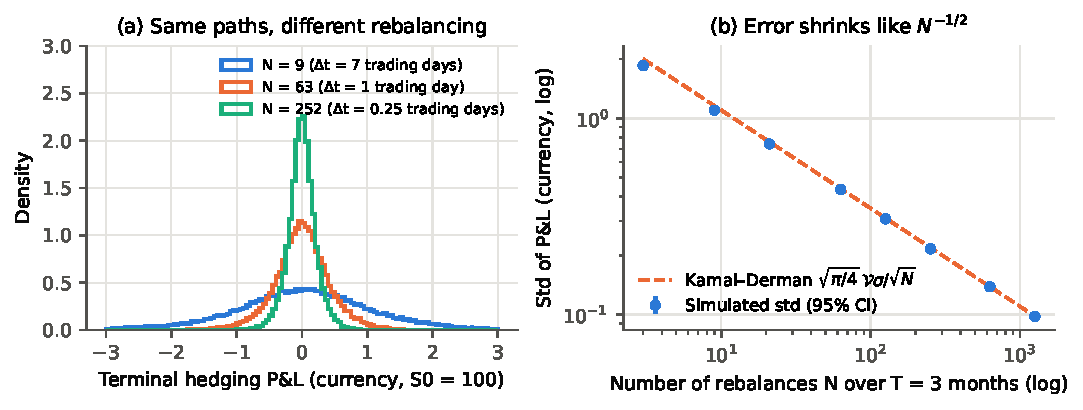
\includegraphics[width=0.84\linewidth]{figures/fig1_frequency.pdf}
\caption{(a) P\&L distributions for three frequencies on the same paths. (b) sd vs $N$ (log--log) with the Kamal--Derman line.}\label{f1}\end{figure}

\textbf{B. Wrong volatility.} The seller prices and hedges at $\sigma_h$ while the true $\sigma=20\%$. With $\sigma_h=10,15,25,30\%$ the mean P\&L is $-1.94,-0.98,+0.99,+1.98$.
Eq.\,(\ref{mis}) predicts $-1.95,-0.98,+0.99,+1.98$, and the mean is the same at $N=63$ and $N=1260$: \emph{more frequent trading does not remove a volatility bias.}
Path by path, the simulated P\&L at $N=1260$ has correlation $0.965$--$0.992$ with (\ref{mis}) (Fig.~\ref{f2}b). The sd also stops falling: at $\sigma_h=25\%$ it is 0.55 at $N=63$ and still
0.35 at $N=1260$, against 0.10 with the correct $\sigma$. Most of the mean error is a \emph{pricing} error. If the premium is charged at the true $\sigma$ but
the delta uses $\sigma_h$, the mean P\&L lies between $-0.02$ and $+0.03$, while the sd is unchanged.
\begin{figure}[t]\centering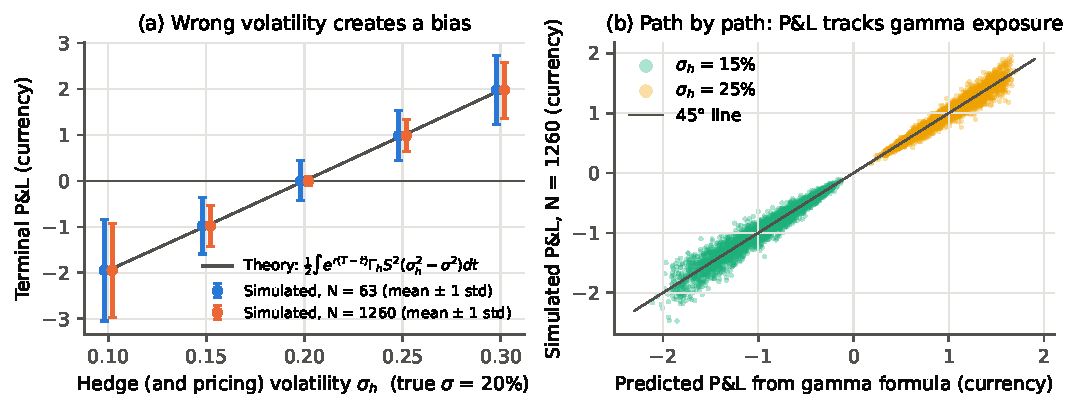
\includegraphics[width=0.84\linewidth]{figures/fig2_misspecification.pdf}
\caption{(a) Mean $\pm1$\,sd of P\&L vs hedge volatility; the line is eq.\,(\ref{mis}). (b) Simulated vs predicted P\&L per path (3{,}000 paths shown).}\label{f2}\end{figure}

\textbf{C. Costs vs frequency.} Expected costs grow with $N$. At 10\,bp they rise from 0.18 ($N=3$) to 1.24 ($N=1260$), so the RMSE curve becomes U-shaped (Fig.~\ref{f3}a).
The RMSE-minimising frequency is $N=1260$ (no cost), 252 (5\,bp), 126 (10\,bp), 63 (20\,bp) and 21 (50\,bp, every 3 trading days). The minimum RMSE rises from 0.10 to 0.58 at 10\,bp, and it is dominated by the
\emph{mean} cost (0.47) rather than by the sd (0.34). Leland's $\sigma_L$ charges for these costs up front. At 10\,bp its mean P\&L is $-0.12$ for \emph{every} $N$, which
matches the simulated cost of the initial purchase plus the final liquidation (0.121). Leland's correction does not cover those two trades.
At $N=1260$ its RMSE is 0.17, against 1.31 for the plain BS delta.
\begin{figure}[t]\centering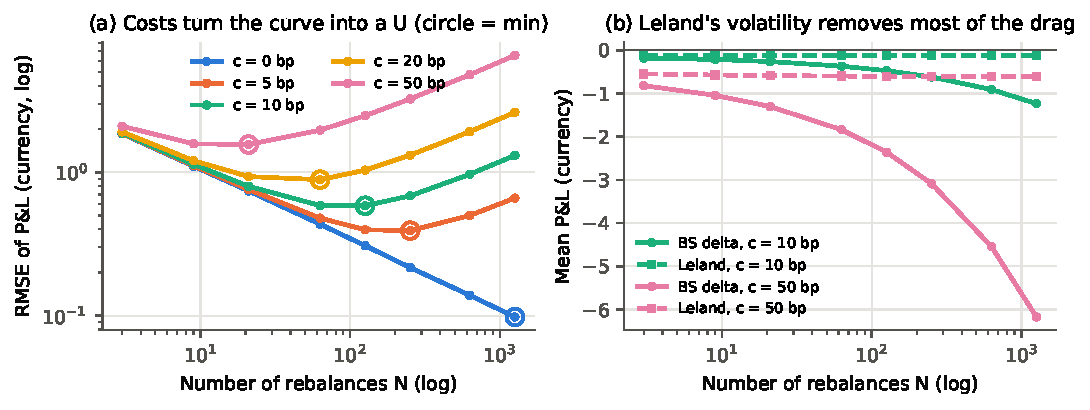
\includegraphics[width=0.84\linewidth]{figures/fig3_costs.pdf}
\caption{(a) RMSE vs $N$ for cost levels 0--50\,bp per side (circle = minimum). (b) Mean P\&L: BS delta (solid) vs Leland (dashed).}\label{f3}\end{figure}

\textbf{D. Asset regimes.} We compare a low-volatility regime ($\sigma=15\%$, $\mu=8\%$) with a high-volatility regime ($\sigma=45\%$, $\mu=12\%$), both simulated and hedged daily.
For the 15\% regime the error sd at the money is 0.32, and for the 45\% regime it is 0.98: the sd scales with $\sigma$ (ratio 3.03), as $\sqrt{\pi/4}\mathcal V\sigma/\sqrt N$ predicts, because ATM vega hardly
depends on $\sigma$. Relative to the premium, out-of-the-money options are much harder to hedge. At $K/S_0=1.2$ the sd is 254\% of a 0.03 premium in the 15\% regime,
against 30\% in the 45\% regime (Fig.~\ref{f4}a). For ATM options hedged daily, the \emph{absolute} error is almost flat in maturity (0.32 for 1--12 months at 15\% volatility), while
the error relative to the premium falls from 17\% to 4\% (Fig.~\ref{f4}b). With 10\,bp costs, the mean cost rises from 0.25 (1 month) to 0.62 (1 year) at 15\% volatility.
\begin{figure}[t]\centering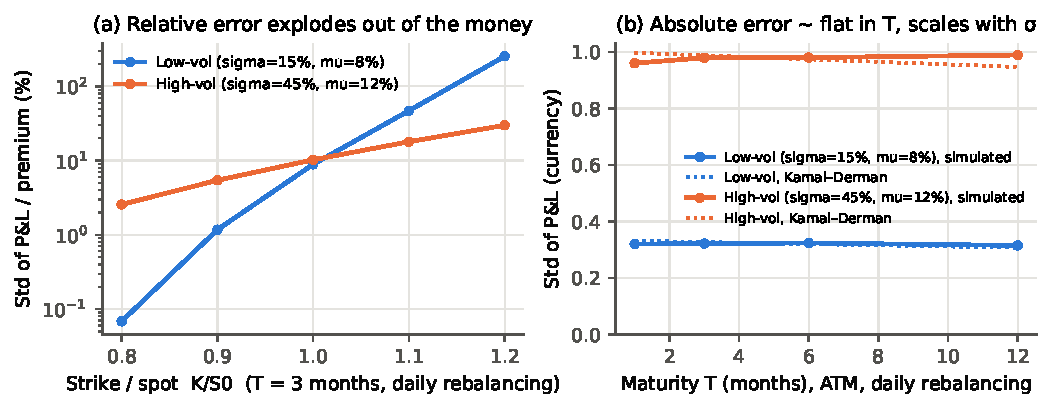
\includegraphics[width=0.84\linewidth]{figures/fig4_regimes.pdf}
\caption{(a) Error sd relative to premium vs moneyness (log scale). (b) Absolute sd vs maturity; dotted = Kamal--Derman.}\label{f4}\end{figure}

\textbf{E. Real data (secondary source; illustration only).} From monthly prices for 2000--2010 (vega-datasets), the annualised volatility is 29\% for IBM, 34\% for MSFT, 39\% for GOOG, 55\% for AAPL and 59\% for AMZN (SE 2--4 points).
Daily adjusted AAPL prices for 2015--17 (plotly/datasets) give 24.3\% (SE 0.8). The drift SEs are 9--19\% per year, so the drift is essentially unestimable, which is harmless
because the hedge does not use it. In the backtest we sell a 63-day ATM AAPL call at a \emph{model} premium (no market quotes), with $\sigma_h$ equal to the trailing 63-day volatility and $r=0.5\%$ assumed. The call is hedged daily
along the actual price path. P\&L/premium ranges from $-115\%$ to $+47\%$. It has correlation 0.87 with $\sigma_h^2-\sigma_{\text{realised}}^2$ over the 380 overlapping windows,
and 0.93 over the 7 non-overlapping windows (Fig.~\ref{f5}), which is consistent with eq.\,(\ref{mis}). The average P\&L ($+3.3\%$ of premium over the overlapping windows, $-1.4\%$ over the non-overlapping ones) is too noisy to interpret.
\begin{figure}[t]\centering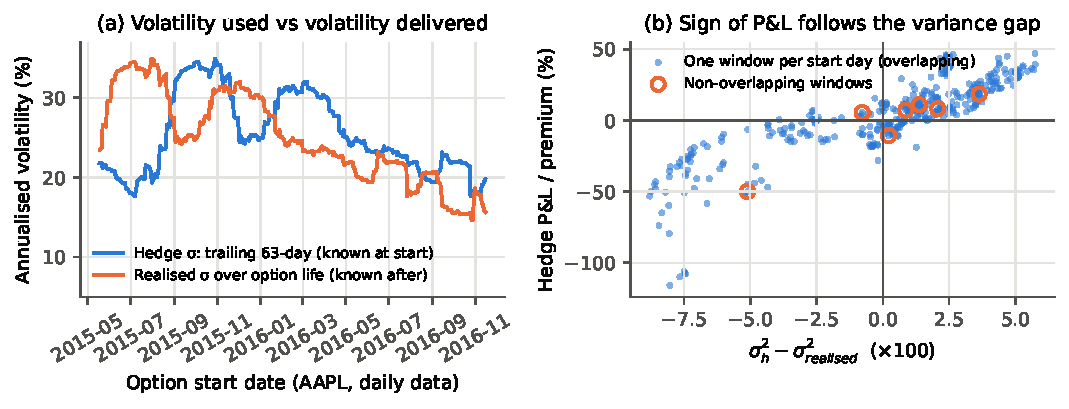
\includegraphics[width=0.84\linewidth]{figures/fig5_realdata.pdf}
\caption{AAPL 2015--17: (a) hedge vs realised volatility; (b) P\&L/premium vs variance gap. Overlapping windows are strongly dependent.}\label{f5}\end{figure}

\section{Conclusions and limitations}
(i) Discrete hedging error is unbiased and has sd $\approx\sqrt{\pi/4}\,\mathcal V\sigma/\sqrt N$: four times more trading halves the error.
(ii) A wrong volatility produces a bias given by the gamma-weighted variance gap (\ref{mis}), and trading more often cannot remove it. Over-estimating $\sigma$ protects the seller on average.
(iii) With proportional costs there is an interior optimal frequency, which moves from every ${\approx}1/4$ day at 5\,bp to every 3 days at 50\,bp. Leland's volatility prices the rebalancing costs but not the set-up and unwind costs.
(iv) Error relative to the premium is largest for OTM, short-dated, low-volatility options.
\emph{Limitations:} constant $\sigma$ and $r$; no jumps, dividends, bid--ask dynamics or market impact; RMSE is only one possible criterion (a utility-based criterion\,\cite{toft} would change the optimum); Monte Carlo SEs
measure sampling error, not model error; the real-data part uses secondary-source prices, model premiums and a short sample.

\begingroup\footnotesize
\renewcommand{\section}[2]{\vspace{2pt}\noindent\textbf{References}\par}
\begin{thebibliography}{99}\setlength{\itemsep}{0pt}
\bibitem{bs} F.~Black, M.~Scholes (1973). The pricing of options and corporate liabilities. \emph{J.\ Political Economy} 81(3), 637--654.
\bibitem{merton} R.\,C.~Merton (1973). Theory of rational option pricing. \emph{Bell J.\ Economics and Management Science} 4(1), 141--183.
\bibitem{be} P.\,P.~Boyle, D.~Emanuel (1980). Discretely adjusted option hedges. \emph{J.\ Financial Economics} 8(3), 259--282.
\bibitem{leland} H.\,E.~Leland (1985). Option pricing and replication with transactions costs. \emph{J.\ Finance} 40(5), 1283--1301.
\bibitem{ks} Y.\,M.~Kabanov, M.\,M.~Safarian (1997). On Leland's strategy of option pricing with transactions costs. \emph{Finance and Stochastics} 1, 239--250.
\bibitem{toft} K.\,B.~Toft (1996). On the mean-variance tradeoff in option replication with transactions costs. \emph{J.\ Financial and Quantitative Analysis} 31(2), 233--263.
\bibitem{ekjs} N.~El~Karoui, M.~Jeanblanc-Picqu\'e, S.\,E.~Shreve (1998). Robustness of the Black and Scholes formula. \emph{Mathematical Finance} 8(2), 93--126.
\bibitem{kd} M.~Kamal, E.~Derman (1999). When you cannot hedge continuously: the corrections of Black--Scholes. \emph{Risk}, Jan.\ 1999 (Goldman Sachs research note).
\bibitem{shreve} S.\,E.~Shreve (2004). \emph{Stochastic Calculus for Finance II: Continuous-Time Models}. Springer.
\bibitem{glass} P.~Glasserman (2004). \emph{Monte Carlo Methods in Financial Engineering}. Springer.
\bibitem{sw} Software: NumPy (Harris et al., \emph{Nature} 585, 2020), SciPy (Virtanen et al., \emph{Nature Methods} 17, 2020), pandas, Matplotlib (Hunter, \emph{CiSE} 9, 2007).
Data: vega-datasets \texttt{stocks.csv} (via \texttt{vega\_datasets} 0.9.0); plotly/datasets \texttt{finance-charts-apple.csv} (see \texttt{data/SOURCES.md}).
\end{thebibliography}
\endgroup
\noindent{\footnotesize\textit{AI assistance:} code, text and figures were drafted with an AI assistant (Claude) and must be checked by the group against the course policy; see \texttt{docs/ai\_disclosure.md}.}
\end{document}
